Описанная модель реализована на языке программирования Java. Реализация сочетает достоинства применения как парадигмы ООП, так и функционального программирования за счет активного использования лямбда-выражений.

% Обозначить, что правильный выбор коллекции - это залог успеха
При проектировании программной реализации было выявлено, что на производительность решения существенное влияние оказывает способ хранения информации о вершинах и дугах. Вариативность способов хранения этой информации зависит от выбранного языка программирования и объема подключаемых библиотек.

% Массивы
Используемый в работах [10], [16], [18] способ хранения информации в массивах является самым простым в реализации. Его использование позволяет наиболее эффективно осуществлять поиск элементов и осуществлять обновление информации о наличествующих в графе вершинах и дугах. Например, как показано в работе [13], изменять значение весовых коэффициентов. Данный способ наиболее эффективно использовать при работе на статическом графе, который не изменяется с течением времени. Использование его в динамически изменяющимся графе приведет к необходимости создания новых экземпляров массивов с последующим заполнением их значений.

% Многомерные массивы
В работе [2] приводится пример использования многомерных массивов. Однако, как описано ранее, данный подход эффективен при неизменяемом числе связей между компонентами графа. Например, если у каждой вершины зафиксировано число дуг, а в процессе преобразований графа моделью изменяется информация о том, в какие именно дуги соединяют вершину с другими вершинами графа. При проектировании модели, в которой число дуг у вершины графа может изменяться, могут создаваться новые вершины и дуги, удаляться ранее созданные, эффективным представляется использование динамических структур данных.

% Списки
Примером динамических структур данных являются связные списки. В работе [4] рассматривается пример их использования. Однако списки допускают хранение одинаковых элементов, что при проектировании описанной графовой модели недопустимо. Модель предусматривает наличие уникальных идентификаторов. Вследствие этого было принято решение об использовании множеств уникальных значений (Set).

Выбранная структура данных может быть реализована по-разному. Выбор реализации влияет на время работы программной реализации модели. С целью проведения экспериментов и получения информации о зависимости времени работы программы от числа элементов графа в реализации предусмотрен модуль для взаимодействия с данными, введенными пользователем:
\begin{enumerate}
    \item модуль определения реализации коллекции Set;
    \item модуль генерации исходных данных.
\end{enumerate}

Модуль определения реализации коллекции Set выполнен для определения временных характеристик работы программной реализации модели при условии использования различных реализаций этой коллекции. Благодаря использованию этого модуля достигается возможность задания конкретной реализации с последующим ее внедрением в исходный код программной реализации модели. Модуль позволяет внедрять как стандартные реализации коллекции Set, так и реализации, хранящиеся в подключаемых библиотеках или самостоятельно реализованные пользователем.

Модуль генерации исходных данных выполнен для сокращения времени на подготовку матрицы трассируемости требований на файлы исходного кода и матрицы зависимостей между файлами исходного кода.

Диаграмма работы выполненной программной реализации приведена на рисунке \ref{fig:application_lifecircle}.

\begin{figure}[H]
    \centering
    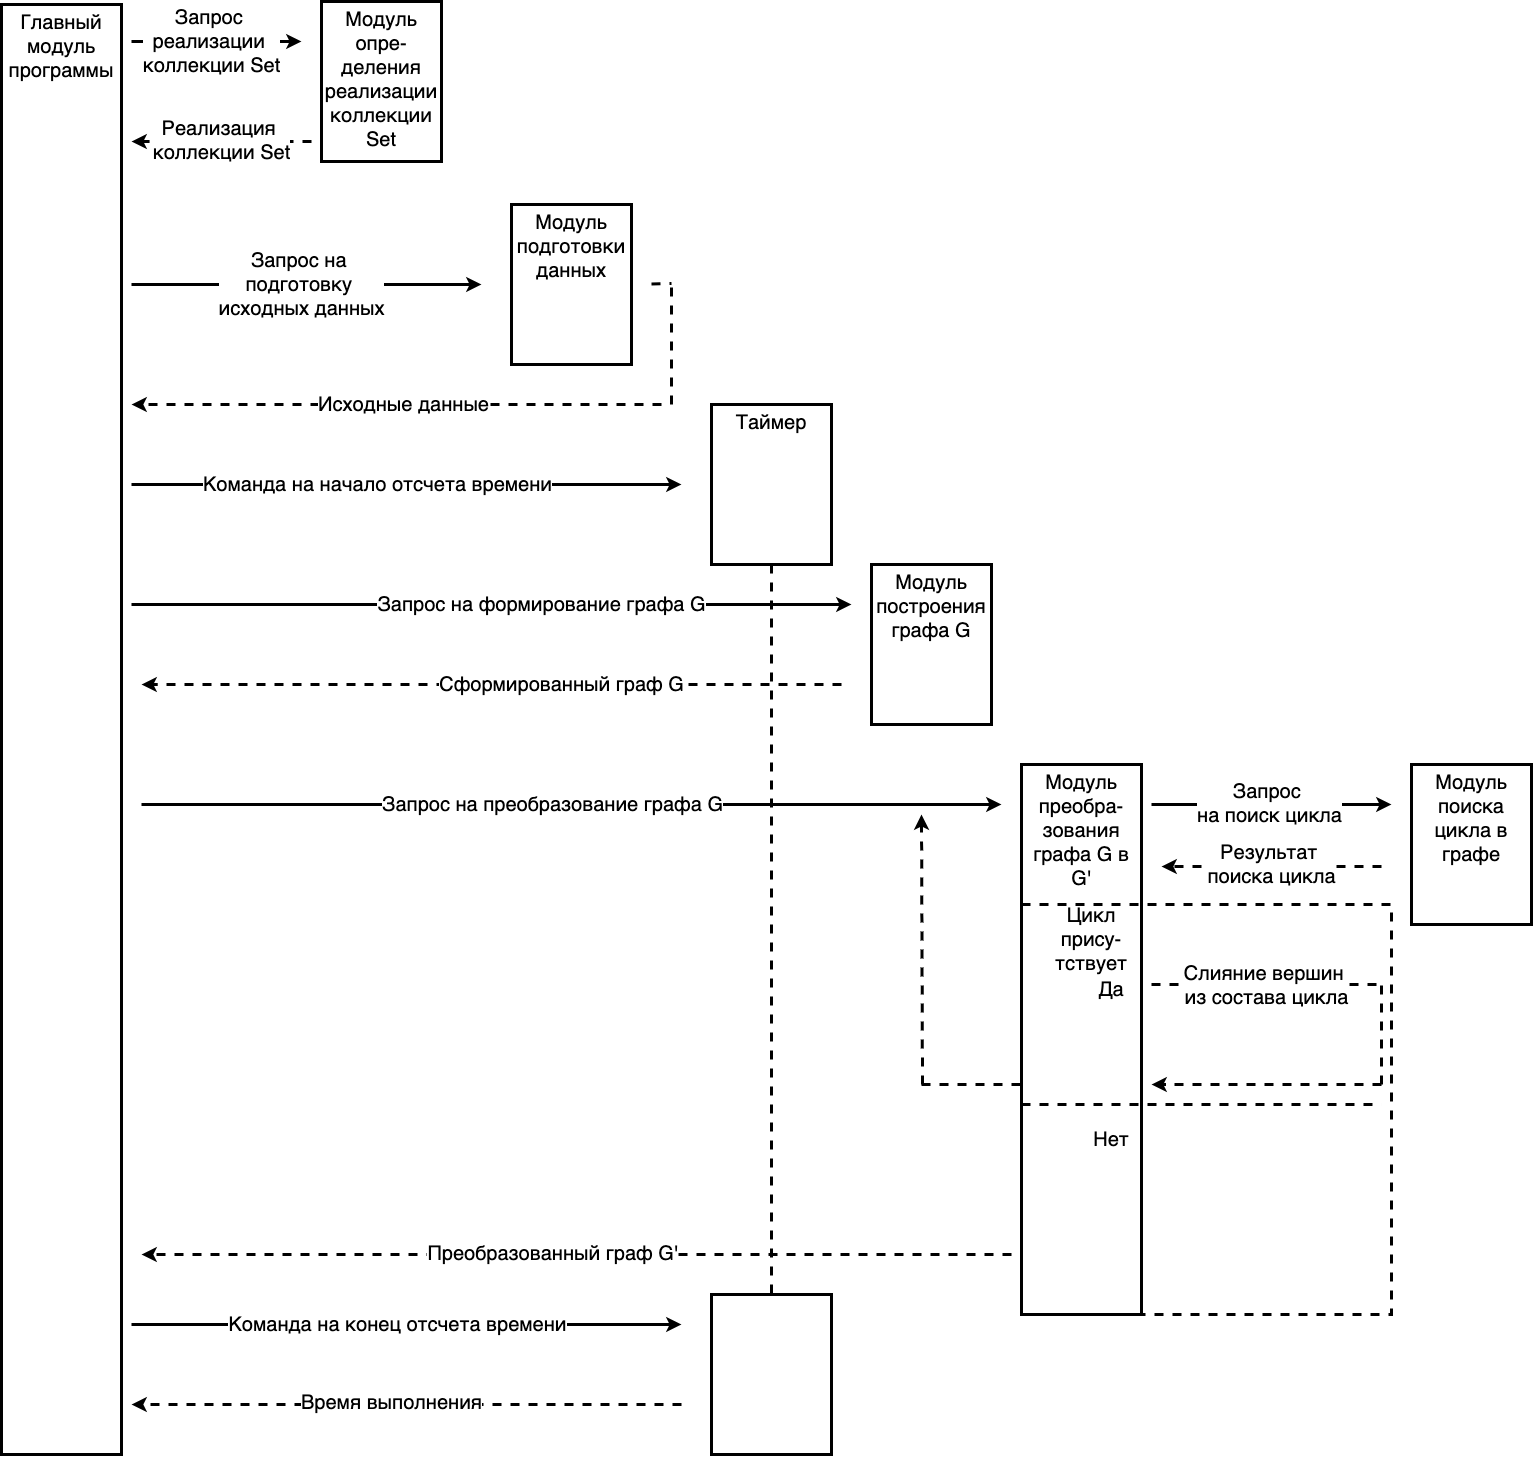
\includegraphics[width=1\textwidth]{application_lifecircle}
    \caption{Диаграмма работы выполненной программной реализации}
    \label{fig:application_lifecircle}
\end{figure}